% todo:
% puddle algorithm: shorten it:
% graphics for slides
% ensure notation is consistent and comprehensive
%

\documentclass{beamer}
\usetheme{Boadilla}
\usepackage{shortcuts}
\usepackage{tikz}
\usepackage{verbatim}
\usepackage[numberedbib]{apacite} 

\title[Abstract Pattern Formation]{A Randomized Approach to Abstract Pattern Formation Fat Robots}
%\subtitle[Errors]{Estimation of numerical errors}
\author[A. Diaz Tolentino \& S. Ramamoorthy]{Armando Jesus Diaz Tolentino \& Sivaramakrishnan Natarajan Ramamoorthy}
\institute[UW]{
	Department of Computer Science\\
	University of Washington\\
	Seattle, Washington \\[1ex]
	\texttt{\{ajdt, sivanr\}@cs.washington.edu}
}
\begin{document}

\begin{frame}
	\titlepage	
\end{frame}
\begin{frame}
	\tableofcontents
\end{frame}

\section{Introduction} 
% justify why the problem is cool, applications!!
\subsection{APF} 
\begin{frame}{Problem Introduction}
	\textbf{Arbitrary Pattern Formation (APF):} 
	\begin{itemize}
		\item Given: A set of $n$ robots arranged arbitrarily on 2D plane 
		\item Goal: form an arbitrary pattern known by all robots \textit{a priori}
		\item Operations: Look, Move, Wait
		\item No explicit communication between robots
	\end{itemize}

	%Related Problems:
	%\begin{itemize}
	% todo: insert graphics to make these problems clear
	%	\item gathering
	%	\item pattern sequencing
	%	\item flocking
	%\end{itemize}
	Applications:
	\begin{itemize}
	% todo: insert graphics to make these problems clear
		\item Simpler generic robots that are composable and configurable vs special purpose monolithic robots
		\item APF used to assign role to robots
	\end{itemize}
\end{frame}

% insert slide for motivations

\subsection{Robot Models} 
\begin{frame}{Robot Models}
	Various Modelling Choices:
	\begin{itemize}
		\item history oblivious, synchronous or ansynchronous 
		\item point vs disk model, transparent vs opaque
		\item compass orientation: 
		\begin{columns}
			\begin{column}{0.5\textwidth}
			\begin{figure}[H]
				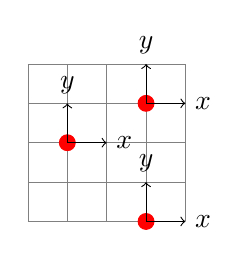
\begin{tikzpicture}[scale=0.5]
					\draw[help lines] (2,2) grid (6,6);
					\draw [red, fill] (5,5) circle [radius=0.2];
					\draw [red, fill] (3,4) circle [radius=0.2];
					\draw [red, fill] (5,2) circle [radius=0.2];
					% axes 
					\draw [->] (5,5) -- (5,6) ;
					\draw [->] (5,5) -- (6,5) ;
					\draw [->] (3,4) -- (3,5) ;
					\draw [->] (3,4) -- (4,4) ;
					\draw [->] (5,2) -- (5,3) ;
					\draw [->] (5,2) -- (6,2) ;
					% lables
					\node[above] at (5,6) {$y$} ;
					\node[right] at (6,5) {$x$} ;
					\node[above] at (3,5) {$y$} ;
					\node[right] at (4,4) {$x$} ;
					\node[above] at (5,3) {$y$} ;
					\node[right] at (6,2) {$x$} ;

				\end{tikzpicture}
			\caption{consistent compass}
			\end{figure}
			\end{column}

			\begin{column}{0.5\textwidth}
			\begin{figure}[H]
				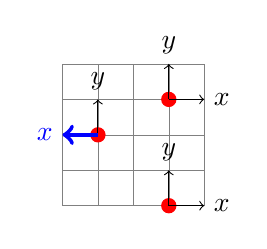
\begin{tikzpicture}[scale=0.45]
					\draw[help lines] (2,2) grid (6,6);
					\draw [red, fill] (5,5) circle [radius=0.2];
					\draw [red, fill] (3,4) circle [radius=0.2];
					\draw [red, fill] (5,2) circle [radius=0.2];
					% axes 
					\draw [->] (5,5) -- (5,6) ;
					\draw [->] (5,5) -- (6,5) ;
					\draw [->] (3,4) -- (3,5) ;
					\draw [blue, ultra thick, ->] (3,4) -- (2,4) ;
					\draw [->] (5,2) -- (5,3) ;
					\draw [->] (5,2) -- (6,2) ;
					% lables
					\node[above] at (5,6) {$y$} ;
					\node[right] at (6,5) {$x$} ;
					\node[above] at (3,5) {$y$} ;
					\node[blue, left] at (2,4) {$x$} ;
					\node[above] at (5,3) {$y$} ;
					\node[right] at (6,2) {$x$} ;
				\end{tikzpicture}
			\caption{OneAxis}
			\end{figure}
			\end{column}
			
			% this section will be left out, due to time constraints
			%\begin{column}{0.3\textwidth}
			%\begin{figure}[H]
			%	\begin{tikzpicture}[scale=0.45]
			%		\draw[help lines] (2,2) grid (7,7);
			%		\draw [red, fill] (5,5) circle [radius=0.2];
			%		\draw [red, fill] (3,4) circle [radius=0.2];
			%		\draw [red, fill] (5,2) circle [radius=0.2];
			%		% axes 
			%		\draw [->] (5,5) -- (4.5,6) ;
			%		\draw [->] (5,5) -- (6,5.4) ;
			%		\draw [->] (3,4) -- (3.2,5) ;
			%		\draw [->] (3,4) -- (4,3.8) ;
			%		\draw [->] (5,2) -- (5,3) ;
			%		\draw [->] (5,2) -- (6,2) ;
			%		% lables
			%		\node[above] at (4.5,6) {$y$} ;
			%		\node[right] at (6,5.4) {$x$} ;
			%		\node[above] at (3.2,5) {$y$} ;
			%		\node[above] at  (4,3.8) {$x$} ;
			%		\node[above] at (5,3) {$y$} ;
			%		\node[right] at (6,2) {$x$} ;
			%	\end{tikzpicture}
			%\caption{Chirality}
			%\end{figure}
			%\end{column}
			
		\end{columns} 
	\end{itemize}
\end{frame}

% won't be used in final presentation
%\begin{frame}{Notation}
%	\begin{itemize}
%		\item We refer to a configuration, $\EE$, as an $n$-tuple of points: $\EE = (x_1,\ldots x_n)$, $x_i \in \RR^2$
%		\item $\EE_i$ is configuration seen by robot $i$
%		\item $\PP$ target pattern robots must form
%		\item global view and local view definitions HERE!! % TODO
%	\end{itemize}
%\end{frame}

\section{Prior Work} 
\subsection{Consistent Compass} 
\begin{frame}{Prior Work: Consistent Compass Trivializes APF}
	Consistent Compass: All robots agree on the orientation of both axes. \\
	\pause
	\textit{Strategy: Total ordering of robots by $y$-coordinate, then $x$-coordinate\cite{flocchini12distrib}.} \\
	\textit{Robot 1 doesn't move. Rest move in order to assigned position.}
	\pause
	\begin{columns}
		\begin{column}{0.5\textwidth}
		\begin{figure}
		\centering
		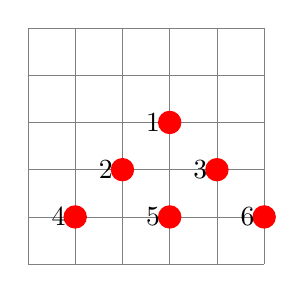
\begin{tikzpicture}[scale=0.60]
			\draw[help lines] (2,2) grid (7,7);

			% circles on l
			\draw [red, fill, ultra thick] (5,5) circle [radius=0.2];
			\draw [red, fill, ultra thick] (4,4) circle [radius=0.2];
			\draw [red, fill, ultra thick] (6,4) circle [radius=0.2];
			\draw [red, fill, ultra thick] (3,3) circle [radius=0.2];
			\draw [red, fill, ultra thick] (5,3) circle [radius=0.2];
			\draw [red, fill, ultra thick] (7,3) circle [radius=0.2];

			% node labels
			\node[left] at (5,5) {$1$} ;
			\node[left] at (4,4) {$2$} ;
			\node[left] at (6,4) {$3$} ;
			\node[left] at (3,3) {$4$} ;
			\node[left] at (5,3) {$5$} ;
			\node[left] at (7,3) {$6$} ;

		\end{tikzpicture}
		\caption{Target Pattern}
		\end{figure}
		\end{column}

		\begin{column}{0.5\textwidth}
		\begin{figure}
		\centering
		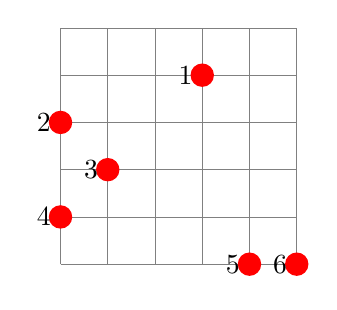
\begin{tikzpicture}[scale=0.60]
			\draw[help lines] (2,2) grid (7,7);

			% circles 
			\draw [red, fill, ultra thick] (2,5) circle [radius=0.2];
			\draw [red, fill, ultra thick] (3,4) circle [radius=0.2];
			\draw [red, fill, ultra thick] (6,2) circle [radius=0.2];
			\draw [red, fill, ultra thick] (2,3) circle [radius=0.2];
			\draw [red, fill, ultra thick] (5,6) circle [radius=0.2];
			\draw [red, fill, ultra thick] (7,2) circle [radius=0.2];

			% node labels
			\node[left] at (2,5) {$2$} ;
			\node[left] at (3,4) {$3$} ;
			\node[left] at (6,2) {$5$} ;
			\node[left] at (2,3) {$4$} ;
			\node[left] at (5,6) {$1$} ;
			\node[left] at (7,2) {$6$} ;
		\end{tikzpicture}
			\caption{Ordering} \label{fig:hi}
		\end{figure}
		\end{column}
	\end{columns}
\end{frame}

\subsection{Impossibility Results} 
\begin{frame}{Prior Work: Good News}
	\begin{theorem} 
		APF is solvable deterministically for odd number of robots with OneAxis even in ASYNC \cite{flocchini08arbitrary}.
	\end{theorem} 
	\begin{columns}
	\begin{column}{0.5\textwidth}
		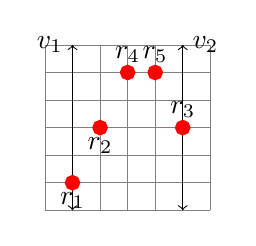
\begin{tikzpicture}[scale=0.35]
			\draw[help lines] (0,0) grid (6,6);

			\draw [<->] (1,0) -- (1,6) ;
			\draw [<->] (5,0) -- (5,6) ;
			% circles
			\draw [red, fill, ultra thick] (1,1) circle [radius=0.2];;
			\draw [red, fill, ultra thick] (2,3) circle [radius=0.2];;
			\draw [red, fill, ultra thick] (5,3) circle [radius=0.2];;
			\draw [red, fill, ultra thick] (3,5) circle [radius=0.2];;
			\draw [red, fill, ultra thick] (4,5) circle [radius=0.2];;

			% node labels
			\node[below] at (1,1) {$r_1$} ;
			\node[below] at (2,3) {$r_2$} ;
			\node[above] at (5,3) {$r_3$} ;
			\node[above] at (3,5) {$r_4$} ;
			\node[above] at (4,5) {$r_5$} ;
			% line labels
			\node[left] at (1,6) {$v_1$} ;
			\node[right] at (5,6) {$v_2$} ;
		\end{tikzpicture}
	\end{column}
	\begin{column}{0.5\textwidth}
		% APF solved
		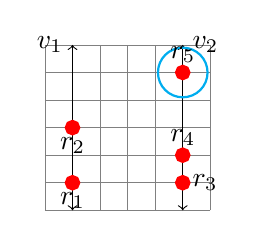
\begin{tikzpicture}[scale=0.35]
			\draw[help lines] (0,0) grid (6,6);
			\draw [<->] (1,0) -- (1,6) ;
			\draw [<->] (5,0) -- (5,6) ;
			% circles
			\draw [red, fill, ultra thick] (1,1) circle [radius=0.2];
			\draw [red, fill, ultra thick] (1,3) circle [radius=0.2];
			\draw [red, fill, ultra thick] (5,1) circle [radius=0.2];
			\draw [red, fill, ultra thick] (5,2) circle [radius=0.2];
			\draw [red, fill, ultra thick] (5,5) circle [radius=0.2];
			\draw [cyan, thick] (5,5) circle [radius=0.9]; % leader circle 
			% node labels
			\node[below] at (1,1) {$r_1$} ;
			\node[below] at (1,3) {$r_2$} ;
			\node[right] at (5,1) {$r_3$} ;
			\node[above] at (5,2) {$r_4$} ;
			\node[above] at (5,5) {$r_5$} ;
			% line labels
			\node[left] at (1,6) {$v_1$} ;
			\node[right] at (5,6) {$v_2$} ;
		\end{tikzpicture}
	\end{column}
	\end{columns}
\end{frame}

\begin{frame}{Prior Work: Bad News}
	\begin{theorem} 
		APF is not solvable deterministically for an even number of robots $ n > 2$ with OneAxis \cite{flocchini12distrib}.
	\end{theorem} 
	\begin{columns}
	\begin{column}{0.5\textwidth}
		\begin{figure}[H]
		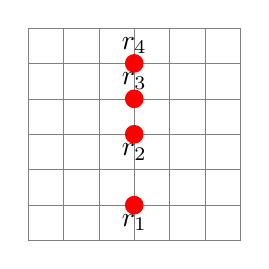
\begin{tikzpicture}[scale=0.45]
			\draw[help lines] (0,0) grid (6,6);
			% circles
			\draw [red, fill, ultra thick] (3,1) circle [radius=0.2];
			\draw [red, fill, ultra thick] (3,3) circle [radius=0.2];
			\draw [red, fill, ultra thick] (3,4) circle [radius=0.2];
			\draw [red, fill, ultra thick] (3,5) circle [radius=0.2];
			% node labels
			\node[below] at (3,1) {$r_1$} ;
			\node[below] at (3,3) {$r_2$} ;
			\node[above] at (3,4) {$r_3$} ;
			\node[above] at (3,5) {$r_4$} ;
		\end{tikzpicture}
		\caption{Target Pattern}
		\end{figure}
	\end{column}
	\begin{column}{0.5\textwidth}
		% bad case
		\begin{figure}[H]
		\centering
		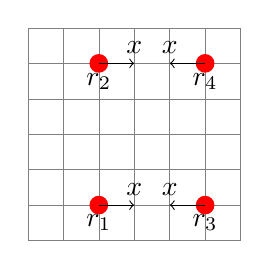
\begin{tikzpicture}[scale=0.45]
			\draw[help lines] (0,0) grid (6,6);
			% circles
			\draw [red, fill, ultra thick] (2,1) circle [radius=0.2];
			\draw [red, fill, ultra thick] (2,5) circle [radius=0.2];
			\draw [red, fill, ultra thick] (5,1) circle [radius=0.2];
			\draw [red, fill, ultra thick] (5,5) circle [radius=0.2];
			% node labels
			\node[below] at (2,1) {$r_1$} ;
			\node[below] at (2,5) {$r_2$} ;
			\node[below] at (5,1) {$r_3$} ;
			\node[below] at (5,5) {$r_4$} ;
			% x axes
			\draw [->] (2,1) -- (3, 1) ;
			\draw [->] (2,5) -- (3, 5) ;
			\draw [->] (5,1) -- (4, 1) ;
			\draw [->] (5,5) -- (4, 5) ;
			% axes labels
			\node[above] at (3, 1) {$x$};
			\node[above] at (3, 5) {$x$};
			\node[above] at (4, 1) {$x$};
			\node[above] at (4, 5) {$x$};
		\end{tikzpicture}
		\caption{Initial Config}
		\end{figure}
	\end{column}
	\end{columns}
\end{frame}


\subsection{Leader Election and APF} 
\begin{frame}{Prior Work: APF and Leader Election}
	\begin{theorem} 
		APF is solvable for $n \geq 3$ robots $\iff$ Leader election problem is solvable.
	\end{theorem} 
	APF $\rightarrow$ leader election: \\
	\pause
	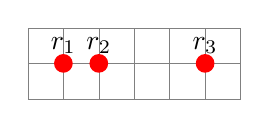
\begin{tikzpicture}[scale=0.45]
		\draw[help lines] (0,0) grid (6,2);
		% circles
		\draw [red, fill, ultra thick] (1,1) circle [radius=0.2];;
		\draw [red, fill, ultra thick] (2,1) circle [radius=0.2];;
		\draw [red, fill, ultra thick] (5,1) circle [radius=0.2];;

		%\node[red, circle, minimum size=0.1cm] at (1,1) {$r_1$} ;
		\node[above] at (1,1) {$r_1$} ;
		\node[above] at (2,1) {$r_2$} ;
		\node[above] at (5,1) {$r_3$} ;
	\end{tikzpicture}

	leader election $\rightarrow$ APF: \\
	\pause
	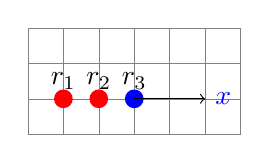
\begin{tikzpicture}[scale=0.45]
		\draw[help lines] (0,0) grid (6,3);
		% circles
		\draw [red, fill, ultra thick] (1,1) circle [radius=0.2];;
		\draw [red, fill, ultra thick] (2,1) circle [radius=0.2];;
		\draw [blue, fill, ultra thick] (3,1) circle [radius=0.2];;

		%\node[red, circle, minimum size=0.1cm] at (1,1) {$r_1$} ;
		\node[above] at (1,1) {$r_1$} ;
		\node[above] at (2,1) {$r_2$} ;
		\node[above] at (3,1) {$r_3$} ;

		% axis of agreement
		\draw [->] (3,1) -- (5,1) ;
		\node[right, blue, thick] at (5,1) {$x$} ;
	\end{tikzpicture}

	Using this insight, our algorithms work to solve leader election first.

\end{frame}

\section{Our Results} 
% insert description of puddle
% demonstrate how odd case works in previous algorithm???

\subsection{PUDDLE: Randomized APF} 
\begin{frame}{Our Work: PUDDLE, a Randomized OneAxis Approach}
	Our Model:
	\begin{itemize}
		\item unit disks, opaque, history oblivious, OneAxis, ASYNC
	\end{itemize}
	3 stages:
	\begin{enumerate}
		\item Move robots to vertical lines $v_1,v_2$
		\item If same number of robots on $v_1$ and on $v_2$, then break symmetry with randomness
		\item Elect leader from current configuration and form $\PP$
	\end{enumerate}
\end{frame}

\begin{frame}{PUDDLE: Part 1}
	\begin{enumerate}
		\item Compute vertical lines $v_1,v_2$ tangent to the convex hull of $\EE$, 
		\item Each robot $i$ moves to $v_1$ or $v_2$ which ever is ``right'' in local view.
	\end{enumerate}
	\begin{columns}
		\begin{column}{0.5\textwidth}
		\begin{figure}
		\centering
		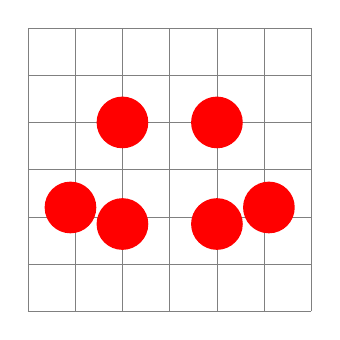
\begin{tikzpicture}[scale=0.60]
			\draw[help lines] (2,1) grid (8,7);

			% circles 
			\draw [red, fill, ultra thick] (4,5) circle [radius=0.5]; % eyes
			\draw [red, fill, ultra thick] (6,5) circle [radius=0.5];
			\draw [red, fill, ultra thick] (2.9,3.2) circle [radius=0.5];% mouth
			\draw [red, fill, ultra thick] (4,2.85) circle [radius=0.5]; 
			\draw [red, fill, ultra thick] (6,2.85) circle [radius=0.5];
			\draw [red, fill, ultra thick] (7.1,3.2) circle [radius=0.5];
			% node labels
			%\node at (4,5) {$r_1$} ;
			%\node at (6,5) {$r_2$} ;
			%\node at (5,4) {$r_3$} ;
			%\node at (2.9,3.2) {$r_4$} ;
			%\node at (4,2.85) {$r_5$} ;
			%\node at (5,2.35) {$r_6$} ;
			%\node at (6,2.85) {$r_7$} ;
			%\node at (7.1,3.2) {$r_8$} ;
		\end{tikzpicture}
		\caption{Target Pattern}
		\end{figure}
		\end{column}

		\begin{column}{0.5\textwidth}
		\begin{figure}
		\centering
		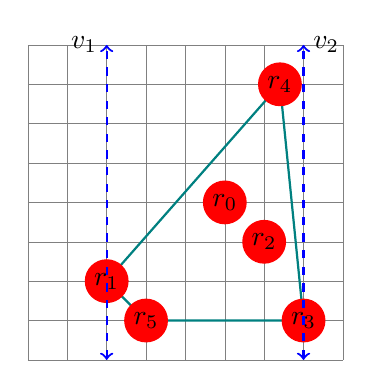
\begin{tikzpicture}[scale=0.50]
			\draw[help lines] (0,0) grid (8,8);

			% shade convex hull
			\draw [teal, thick] (2,2) -- (6.4, 7) -- (7,1) -- (3,1) -- (2,2) ;
			% circles 
			\draw [red, fill, ultra thick] (2,2) circle [radius=0.5]; 
			\draw [red, fill, ultra thick] (6,3) circle [radius=0.5];
			\draw [red, fill, ultra thick] (5,4) circle [radius=0.5]; 
			\draw [red, fill, ultra thick] (6.4,7) circle [radius=0.5]; 
			\draw [red, fill, ultra thick] (3,1) circle [radius=0.5];
			\draw [red, fill, ultra thick] (7,1) circle [radius=0.5];

			% lines for $v_1$ and $v_2$
			\draw [blue, dashed, thick, <->] (2,0) -- (2,8) ;
			\draw [blue, dashed, thick, <->] (7,0) -- (7,8) ;
			% labels for lines
			\node[left] at (2,8) {$v_1$} ;
			\node[right] at (7,8) {$v_2$} ;
			% labels for robots
			\node at (2,2) {$r_1$};
			\node at (6,3) {$r_2$};
			\node at (5,4) {$r_0$};
			\node at (6.4,7) {$r_4$};
			\node at (3,1) {$r_5$};
			\node at (7,1) {$r_3$};

		\end{tikzpicture}
			\caption{Convex Hull} \label{fig:hi}
		\end{figure}
		\end{column}
	\end{columns}
\end{frame}


\begin{frame}{PUDDLE: Part 2}
	\begin{enumerate}
		% SHOW IN PICTURE: We refer to $L$ as the region on the same side of $l$ with respect to 
		% 		the line $m$, and refer to $R$ similarly .
		\item Let $r$ refer to the line on the side with the majority of robots, and $l$ refer to the side
		with a minority of robots.
		\item If a side has majority of robots, this side determines the x-axis direction.
		\item If  no majority on either side, compute center line $m$ 
			with some probability $\frac{1}{n}$ each robot moves to the center line $m$. 
	\end{enumerate}
	\begin{columns}
		\begin{column}{0.5\textwidth}
		\begin{figure}
		\centering
		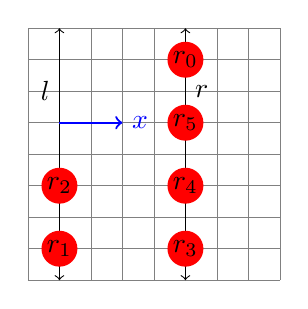
\begin{tikzpicture}[scale=0.40]
			\draw[help lines] (0,0) grid (8,8);

			\draw [<->] (1,0) -- (1,8) ;
			\draw [<->] (5,0) -- (5,8) ;
			% circles on l
			\draw [red, fill, ultra thick] (1,1) circle [radius=0.5];
			\draw [red, fill, ultra thick] (1,3) circle [radius=0.5];

			% circles on r
			\draw [red, fill, ultra thick] (5,7) circle [radius=0.5];
			\draw [red, fill, ultra thick] (5,1) circle [radius=0.5];
			\draw [red, fill, ultra thick] (5,3) circle [radius=0.5];
			\draw [red, fill, ultra thick] (5,5) circle [radius=0.5];

			% node labels
			\node at (5,7) {$r_0$} ;
			\node at (1,1) {$r_1$} ;
			\node at (1,3) {$r_2$} ;
			\node at (5,1) {$r_3$} ;
			\node at (5,3) {$r_4$} ;
			\node at (5,5) {$r_5$} ;

			% line labels
			\node[left] at (1,6) {$l$} ;
			\node[right] at (5,6) {$r$} ;

			% arrow for x axis
			\draw [blue, thick,->] (1,5) -- (3,5) ;
			\node[blue, right] at (3,5) {$x$};

			
		\end{tikzpicture}
		\caption{already asymmetric}
		\end{figure}
		\end{column}

		\begin{column}{0.5\textwidth}
		\begin{figure}
		\centering
		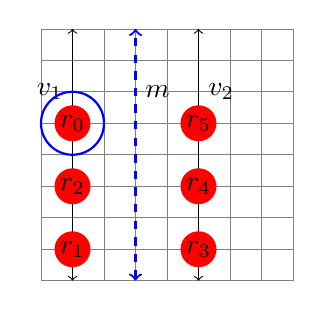
\begin{tikzpicture}[scale=0.40]
			\draw[help lines] (0,0) grid (8,8);

			\draw [<->] (1,0) -- (1,8) ;
			\draw [<->] (5,0) -- (5,8) ;
			\draw [dashed, thick, blue,<->] (3,0) -- (3,8) ;
			% circles on l
			
			\draw [red, fill, ultra thick] (1,5) circle [radius=0.5];
			\draw [red, fill, ultra thick] (1,1) circle [radius=0.5];
			\draw [red, fill, ultra thick] (1,3) circle [radius=0.5];

			% circles on r
			\draw [red, fill, ultra thick] (5,1) circle [radius=0.5];
			\draw [red, fill, ultra thick] (5,3) circle [radius=0.5];
			\draw [red, fill, ultra thick] (5,5) circle [radius=0.5];

			% node labels
			\node at (1,5) {$r_0$} ;
			\node at (1,1) {$r_1$} ;
			\node at (1,3) {$r_2$} ;
			\node at (5,1) {$r_3$} ;
			\node at (5,3) {$r_4$} ;
			\node at (5,5) {$r_5$} ;

			% line labels
			\node[left] at (1,6) {$v_1$} ;
			\node[right] at (5,6) {$v_2$} ;
			\node[right] at (3,6) {$m$} ;

			% r_0 moves 
			\draw [blue, thick] (1,5) circle [radius=1];
			%\draw [blue, thick,->, right] (1,5) -- (3,5) ;
			%\node[right, blue] at (3,5) {$x$} ;

			
		\end{tikzpicture}
			\caption{breaking symmetry} \label{fig:hi}
		\end{figure}
		\end{column}
	\end{columns}
\end{frame}

% NOTE: duplicate slide to fake animation
\begin{frame}{PUDDLE: Part 2}
	\begin{enumerate}
		% SHOW IN PICTURE: We refer to $L$ as the region on the same side of $l$ with respect to 
		% 		the line $m$, and refer to $R$ similarly .
		\item Let $r$ refer to the line on the side with the majority of robots, and $l$ refer to the side
		with a minority of robots.
		\item If a side has majority of robots, this side determines the x-axis direction.
		\item If  no majority on either side, compute center line $m$ 
			with some probability $\frac{1}{n}$ each robot moves to the center line $m$. 
	\end{enumerate}
	\begin{columns}
		\begin{column}{0.5\textwidth}
		\begin{figure}
		\centering
		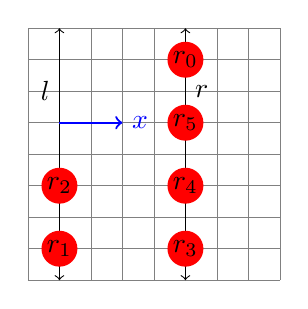
\begin{tikzpicture}[scale=0.40]
			\draw[help lines] (0,0) grid (8,8);

			\draw [<->] (1,0) -- (1,8) ;
			\draw [<->] (5,0) -- (5,8) ;
			% circles on l
			\draw [red, fill, ultra thick] (1,1) circle [radius=0.5];
			\draw [red, fill, ultra thick] (1,3) circle [radius=0.5];

			% circles on r
			\draw [red, fill, ultra thick] (5,7) circle [radius=0.5];
			\draw [red, fill, ultra thick] (5,1) circle [radius=0.5];
			\draw [red, fill, ultra thick] (5,3) circle [radius=0.5];
			\draw [red, fill, ultra thick] (5,5) circle [radius=0.5];

			% node labels
			\node at (5,7) {$r_0$} ;
			\node at (1,1) {$r_1$} ;
			\node at (1,3) {$r_2$} ;
			\node at (5,1) {$r_3$} ;
			\node at (5,3) {$r_4$} ;
			\node at (5,5) {$r_5$} ;

			% line labels
			\node[left] at (1,6) {$l$} ;
			\node[right] at (5,6) {$r$} ;

			% arrow for x axis
			\draw [blue, thick,->] (1,5) -- (3,5) ;
			\node[blue, right] at (3,5) {$x$};

			
		\end{tikzpicture}
		\caption{already asymmetric}
		\end{figure}
		\end{column}

		\begin{column}{0.5\textwidth}
		\begin{figure}
		\centering
		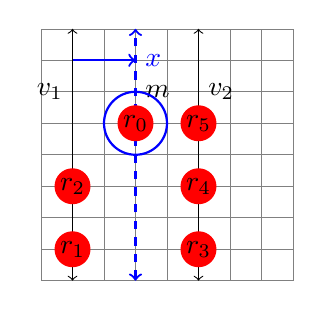
\begin{tikzpicture}[scale=0.40]
			\draw[help lines] (0,0) grid (8,8);

			\draw [<->] (1,0) -- (1,8) ;
			\draw [<->] (5,0) -- (5,8) ;
			\draw [dashed, thick, blue,<->] (3,0) -- (3,8) ;
			% circles on l
			
			\draw [red, fill, ultra thick] (1,1) circle [radius=0.5];
			\draw [red, fill, ultra thick] (1,3) circle [radius=0.5];

			% circle on m
			\draw [red, fill, ultra thick] (3,5) circle [radius=0.5];

			% circles on r
			\draw [red, fill, ultra thick] (5,1) circle [radius=0.5];
			\draw [red, fill, ultra thick] (5,3) circle [radius=0.5];
			\draw [red, fill, ultra thick] (5,5) circle [radius=0.5];

			% node labels
			\node at (3,5) {$r_0$} ;
			\node at (1,1) {$r_1$} ;
			\node at (1,3) {$r_2$} ;
			\node at (5,1) {$r_3$} ;
			\node at (5,3) {$r_4$} ;
			\node at (5,5) {$r_5$} ;

			% line labels
			\node[left] at (1,6) {$v_1$} ;
			\node[right] at (5,6) {$v_2$} ;
			\node[right] at (3,6) {$m$} ;

			% r_0 moves 
			\draw [blue, thick] (3,5) circle [radius=1];
			\draw [blue, thick,->, right] (1,7) -- (3,7) ;
			\node[right, blue] at (3,7) {$x$} ;

			
		\end{tikzpicture}
			\caption{breaking symmetry} \label{fig:hi}
		\end{figure}
		\end{column}
	\end{columns}
\end{frame}

\begin{frame}{PUDDLE: Part 3}
	\begin{enumerate}
		\item In finite time, either all robots are on $m$,
		or consensus reached on direction for $x$ axis.
		\item If all the robots are on $m$, then we have solved the leader election problem, and 
		can form the arbitrary pattern trivially.
		\item If x-axis determined, then leader is top-robot on $l$, and form pattern first using
		all bots in $l$, then $m$, and $r$.
	\end{enumerate}
		
		%\begin{figure}
		%\begin{tikzpicture}[scale=0.40]
		%	\draw[help lines] (0,0) grid (8,8);
%
%			\draw [<->] (1,0) -- (1,8) ;
%			\draw [<->] (5,0) -- (5,8) ;
%			\draw [dashed, thick, blue,<->] (3,0) -- (3,8) ;
%			% circles on l
%			
%			\draw [red, fill, ultra thick] (1,1) circle [radius=0.5];
%			\draw [red, fill, ultra thick] (1,3) circle [radius=0.5];
%
%			% circle on m
%			\draw [red, fill, ultra thick] (3,5) circle [radius=0.5];
%
%			% circles on r
%			\draw [red, fill, ultra thick] (5,1) circle [radius=0.5];
%			\draw [red, fill, ultra thick] (5,3) circle [radius=0.5];
%			\draw [red, fill, ultra thick] (5,5) circle [radius=0.5];
%
%			% node labels
%			\node at (3,5) {$3$} ;
%			\node at (1,1) {$2$} ;
%			\node at (1,3) {$1$} ;
%			\node at (5,1) {$6$} ;
%			\node at (5,3) {$5$} ;
%			\node at (5,5) {$4$} ;
%
%			% line labels
%			\node[left] at (1,6) {$v_1$} ;
%			\node[right] at (5,6) {$v_2$} ;
%			\node[right] at (3,6) {$m$} ;
%		\end{tikzpicture}
%		\caption{Ordering}
%		\end{figure}
\end{frame}

\begin{frame}{PUDDLE: Guarantees }
	\begin{itemize}
		\item x-axis consensus  only fails if:
			\begin{itemize}
				\item No robots move $Pr = (1 - \frac{1}{k})^{k} \leq \frac{1}{e} \approx 0.37$
				\item The same number of robots move from each side:
					$$\sum_{i=1}^{k}{((\frac{1}{k})^i (\frac{k-1}{k})^{k-i} {k\choose i})^2} \leq 0.20$$
			\end{itemize}
		\item Probability of success is at least $0.43$. Consensus in 3 rounds (in expectation).
		\item Algorithm works for Disk model (prev result for point model)
		\item Guaranteed collision free (details in report)
	\end{itemize}
\end{frame}

\subsection{Result using SEC} 
\begin{frame}{Revisiting APF with SEC}
\begin{theorem}
There exists no deterministic algorithm that solves the Leader Election Problem, even with chirality assumption.
\end{theorem}
\pause
Idea: Find an initial configuration such that every robot's local view is the same. 
\pause
\begin{figure}[ht!]
\centering
		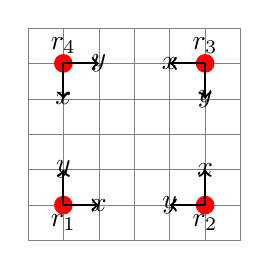
\begin{tikzpicture}[scale=0.45]
			\draw[help lines] (0,0) grid (6,6);

			% circles
			\draw [red, fill, ultra thick] (1,1) circle [radius=0.2];;
			\draw [red, fill, ultra thick] (5,1) circle [radius=0.2];;
			\draw [red, fill, ultra thick] (5,5) circle [radius=0.2];;
			\draw [red, fill, ultra thick] (1,5) circle [radius=0.2];;

			% axes
			\draw[thick, ->] (1,1) -- (1,2) ; % robot 1
			\draw[thick, ->] (1,1) -- (2,1) ; 
			\node at (1,2) {$y$} ;
			\node at (2,1) {$x$} ;
			\draw[thick, ->] (5,1) -- (4,1) ; % robot 2
			\draw[thick, ->] (5,1) -- (5,2) ; 
			\node at (4,1) {$y$} ;
			\node at (5,2) {$x$} ;
			\draw[thick, ->] (5,5) -- (5,4) ; % robot 3
			\draw[thick, ->] (5,5) -- (4,5) ; 
			\node at (5,4) {$y$} ;
			\node at (4,5) {$x$} ;
			\draw[thick, ->] (1,5) -- (2,5) ; % robot 4
			\draw[thick, ->] (1,5) -- (1,4) ; 
			\node at (2,5) {$y$} ;
			\node at (1,4) {$x$} ;

			%\node[red, circle, minimum size=0.1cm] at (1,1) {$r_1$} ;
			\node[below] at (1,1) {$r_1$} ;
			\node[below] at (5,1) {$r_2$} ;
			\node[above] at (5,5) {$r_3$} ;
			\node[above] at (1,5) {$r_4$} ;

			% draw circles at positions desired
			%\draw [red, ultra thick] (0,0)
			%\draw (1,1) -- (5,1) -- (5,5) -- (1,5) -- (1,1);
		\end{tikzpicture}
	%\end{float}
\end{figure}
\end{frame}

\begin{frame}{An SEC Randomized Algorithm for APF}
Some Notation:
\begin{itemize}
\item $SEC$ - A circle of minimal radius enclosing the given points 
\item $SEC_p$ - A circle of minimal radius enclosing the given points, centered at $p$
\end{itemize}
\pause
Basic Idea:
\begin{itemize}
\item A trivial observation: If there is only one robot on the circumference of $SEC_p(\text{Robots})$, the robot on the circumference can be elected the leader. 
\item Any underlying assumption? - Every robot sees every other robot 
\end{itemize}
\end{frame}

\begin{frame}
Some Notation:
\begin{itemize}
\item $SEC$ - A circle of minimal radius enclosing the given points 
\item $SEC_p$ - A circle of minimal radius enclosing the given points, centered at $p$
\end{itemize}

Basic Idea:
\begin{figure}[H]
				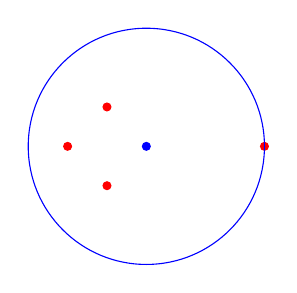
\begin{tikzpicture}[scale=0.5]
					\draw [red, fill] (9,5) circle [radius=0.1];
					\draw [red, fill] (4,5) circle [radius=0.1];
					\draw [red, fill] (5,6) circle [radius=0.1];
					\draw [red, fill] (5,4) circle [radius=0.1];

					\draw [blue, fill] (6,5) circle [radius=0.1];					
					
					\draw [blue] (6,5) circle [radius = 3];
				\end{tikzpicture}
			\end{figure}
\end{frame}

\begin{frame}{Algorithm Continued....}
\begin{itemize}
\item Let us assume that every robot gets to see every other robot
\pause
\item Compute $p=$\emph{CG(Robots)} - everyone agrees!!
\item Compute $SEC_p(\text{Robots})$
\item Robots on $SEC_p$ contest, others move outside $SEC_p$
\end{itemize}
\end{frame}

\begin{frame}
\begin{figure}[H]
				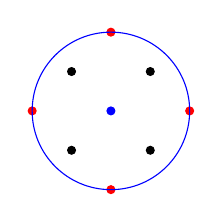
\begin{tikzpicture}[scale=0.5]
					\draw [red, fill] (7,5) circle [radius=0.1];
					\draw [red, fill] (3,5) circle [radius=0.1];
					\draw [red, fill] (5,7) circle [radius=0.1];
					\draw [red, fill] (5,3) circle [radius=0.1];

					\draw [blue, fill] (5,5) circle [radius=0.1];					
					
					\draw [black, fill] (6,6) circle [radius=0.1];
					\draw [black, fill] (6,4) circle [radius=0.1];
					\draw [black, fill] (4,4) circle [radius=0.1];
					\draw [black, fill] (4,6) circle [radius=0.1];
					
					\draw [blue] (5,5) circle [radius = 2];
				\end{tikzpicture}
			\end{figure}
\end{frame}

\begin{frame}
\begin{figure}[H]
				\begin{tikzpicture}[scale=0.5]
					\draw [red, fill] (7,5) circle [radius=0.1];
					\draw [red, fill] (3,5) circle [radius=0.1];
					\draw [red, fill] (5,7) circle [radius=0.1];
					\draw [red, fill] (5,3) circle [radius=0.1];

					\draw [blue, fill] (5,5) circle [radius=0.1];					
					
					\draw [black, fill] (9,9) circle [radius=0.1];
					\draw [black, fill] (9,1) circle [radius=0.1];
					\draw [black, fill] (1,9) circle [radius=0.1];
					\draw [black, fill] (1,1) circle [radius=0.1];
					
					\draw [blue] (5,5) circle [radius = 2];

				\end{tikzpicture}
			\end{figure}
\end{frame}

\begin{frame}{Algorithm Continued....}
\begin{itemize}
\item Robots on $SEC_p$ more outward with probability $\frac{1}{|\text{number of robots on $SEC$ }|}$
\item Robots compute $SEC_p(\text{Contesting Robots})$
\item If only one robot on $SEC_p$, elect that to be the leader.
\item Otherwise one more round to elect.
\end{itemize}
\end{frame}

\begin{frame}
\begin{figure}[H]
				\begin{tikzpicture}[scale=0.5]
					\draw [red, fill] (7,5) circle [radius=0.1];
					\draw [red, fill] (3,5) circle [radius=0.1];
					\draw [red, fill] (5,7) circle [radius=0.1];
					\draw [red, fill] (5,3) circle [radius=0.1];

					\draw [blue, fill] (5,5) circle [radius=0.1];					
					
					\draw [black, fill] (9,9) circle [radius=0.1];
					\draw [black, fill] (9,1) circle [radius=0.1];
					\draw [black, fill] (1,9) circle [radius=0.1];
					\draw [black, fill] (1,1) circle [radius=0.1];
					
					\draw [blue] (5,5) circle [radius = 2];
					
					\draw [->] (7,5) -- (8,6.32) ;
					\draw [-] (7,3) -- (7,7) ;
				\end{tikzpicture}
			\end{figure}
\end{frame}

\begin{frame}
\begin{figure}[H]
				\begin{tikzpicture}[scale=0.5]
					\draw [red, fill] (8,6.32) circle [radius=0.1];
					\draw [black, fill] (3,5) circle [radius=0.1];
					\draw [black, fill] (5,7) circle [radius=0.1];
					\draw [black, fill] (5,3) circle [radius=0.1];

					\draw [blue, fill] (5,5) circle [radius=0.1];					
					
					\draw [black, fill] (9,9) circle [radius=0.1];
					\draw [black, fill] (9,1) circle [radius=0.1];
					\draw [black, fill] (1,9) circle [radius=0.1];
					\draw [black, fill] (1,1) circle [radius=0.1];
					
					\draw [blue] (5,5) circle [radius = 3.27];
				\end{tikzpicture}
			\end{figure}
\end{frame}

\begin{frame}{Ensuring every robot sees every other robot}
\begin{itemize}
\item Check if you can see every other robot, If $YES$, do nothing!! 
\pause
\item If $NO$, do the following...
\item Compute $SEC_p(\text{Local View})$
\item Move to circumference of $SEC_p$
\end{itemize}
\end{frame}

\section{Open Problems and Future Work} 
\begin{frame}{Open Problems and Future Work}
Open Problems:
\begin{itemize}
\item Taking up too much space!!! Can one bound it? 
\pause
\item What if there are obstacles in the plane - look at obstacles as line segments on $\mathbb{R}^2$
\end{itemize}
\pause
Future Directions:
\begin{itemize}
	\item Two randomized algorithms for circle formation; more space efficient
\end{itemize}
\end{frame}

\begin{frame}{Summary}
	\begin{itemize}
		\item Prior work solves APF for odd number of robots with OneAxis assumption.
		\pause
		\item Our work:
			\begin{itemize}
				\item APF solved for even robots with OneAxis
				\item APF solved with no axis assumptions; less space efficient
			\end{itemize}
	\end{itemize}
\end{frame}

\begin{frame}{Thank You}
Questions?
\begin{figure}[ht!]
\centering
\includegraphics[width=90mm]{qa_img.jpg}
\end{figure}
\end{frame}

\begin{frame}{References}
%\begin{frame}[allowframebreaks]{References}
\bibliographystyle{apacite} 
\bibliography{presentation}
\end{frame}

\end{document}

%todo
% practice
